\documentclass[conference]{IEEEtran}
\IEEEoverridecommandlockouts
% The preceding line is only needed to identify funding in the first footnote. If that is unneeded, please comment it out.
\usepackage{cite}
\usepackage{amsmath,amssymb,amsfonts}
\usepackage{algorithmic}
\usepackage{graphicx}
\usepackage[caption=false,font=footnotesize]{subfig}
\usepackage{textcomp}
\usepackage{xcolor}
\usepackage{booktabs}
\def\BibTeX{{\rm B\kern-.05em{\sc i\kern-.025em b}\kern-.08em
    T\kern-.1667em\lower.7ex\hbox{E}\kern-.125emX}}
\begin{document}

\title{Conference Paper Title*\\
{\footnotesize \textsuperscript{*}Note: Sub-titles are not captured in Xplore and
should not be used}
\thanks{Identify applicable funding agency here. If none, delete this.}
}

\author{\IEEEauthorblockN{1\textsuperscript{st} Given Name Surname}
\IEEEauthorblockA{\textit{dept. name of organization (of Aff.)} \\
\textit{name of organization (of Aff.)}\\
City, Country \\
email address or ORCID}
\and
\IEEEauthorblockN{2\textsuperscript{nd} Given Name Surname}
\IEEEauthorblockA{\textit{dept. name of organization (of Aff.)} \\
\textit{name of organization (of Aff.)}\\
City, Country \\
email address or ORCID}
\and
\IEEEauthorblockN{3\textsuperscript{rd} Given Name Surname}
\IEEEauthorblockA{\textit{dept. name of organization (of Aff.)} \\
\textit{name of organization (of Aff.)}\\
City, Country \\
email address or ORCID}
\and
\IEEEauthorblockN{4\textsuperscript{th} Given Name Surname}
\IEEEauthorblockA{\textit{dept. name of organization (of Aff.)} \\
\textit{name of organization (of Aff.)}\\
City, Country \\
email address or ORCID}
\and
\IEEEauthorblockN{5\textsuperscript{th} Given Name Surname}
\IEEEauthorblockA{\textit{dept. name of organization (of Aff.)} \\
\textit{name of organization (of Aff.)}\\
City, Country \\
email address or ORCID}
\and
\IEEEauthorblockN{6\textsuperscript{th} Given Name Surname}
\IEEEauthorblockA{\textit{dept. name of organization (of Aff.)} \\
\textit{name of organization (of Aff.)}\\
City, Country \\
email address or ORCID}
}

\maketitle

\begin{abstract}
This document is a model and instructions for \LaTeX.
This and the IEEEtran.cls file define the components of your paper [title, text, heads, etc.]. *CRITICAL: Do Not Use Symbols, Special Characters, Footnotes, 
or Math in Paper Title or Abstract.
\end{abstract}

\begin{IEEEkeywords}
component, formatting, style, styling, insert
\end{IEEEkeywords}

\section{Introduction}
The construction sector has long been one of the least automated of the major industries, and robots are now beginning to move from controlled factories onto construction sites.  Robots now take on a wide range of construction tasks, from three-dimensional concrete printing, bricklaying, and steel welding and assembly, through material transport, excavation, and drilling, to panel and facade installation, painting, plastering, tiling, surveying, inspection, and demolition, with one recent review screening 375 studies published between 2023 and 2025 alone~\cite{Gharbia2020-ml,Xu2026-cr}. The platforms carrying out this work vary widely in form, spanning wheeled and legged robots, gantry printers, and wearable exoskeletons. Their arrival is driven less by novelty than by necessity, since construction ranks among the least productive industries~\cite{Rathnayake2023-xt}, and moving robots into these tasks also removes workers from hazardous conditions. A large share of these tasks are performed by mobile robots that must travel across the site and position themselves at the work location. As a result, before a robot can transport a load, inspect a structure, or finish a surface, it must first physically reach the area where the work is to be done. Construction sites are unstructured, cluttered, and constantly changing~\cite{Xu2026-cr}, and the barriers reported in the literature are dominated by the physical environment rather than by any shortfall in what the robot can do.  Across surveyed studies, limitation in workspace is the single most cited challenge, reported in around 43\% of the papers that document barriers, ahead of structural integrity and the complexity of coordinating robot movement~\cite{Gharbia2020-ml}. Field assessments of active sites reveal several recurring constraints, among them human density, surface unevenness, accessibility, lighting variation, and dynamic clutter, and these constraints are not equal in weight. Accessibility is the binding one, because the others only matter in regions the robot can already reach, and once a region is reachable they become ordinary engineering problems with well-understood mitigations.



Reconfigurable and modular platforms tackle constrained spaces by changing their own geometry, splitting or folding so the robot can pass through gaps a fixed body could not~\cite{CONCERT,9817632, prabakaran2017htetro}, although this adds mechanical joints and control complexity. Newer navigation stacks add learned perception, multi-sensor fusion, and online path planners that replan around obstacles as they appear. These methods make a robot move through a site more reliably, but they demand heavy sensing and computation, and they operate only after the robot is already on site. What these responses have in common is that they act on the robot or on its perception rather than on the site itself.

The idea of robot inclusivity, meaning the extent to which an environment admits a given robot, has been raised in earlier work~\cite{robot_inclusivity_2013,buildings14051193}. The methods proposed so far are largely manual, in which a person walks the site and judges suitability by eye, and such assessment neither scales across many floors and fleets of different robots nor forecasts the effect of a proposed change. Closer to an automated measure, an inclusivity-style index has been proposed for illumination conditions~\cite{zeng2024riilux}, and a companion 






index scores floor surface unevenness~\cite{borusu2024rilsu}, yet neither produces an accessibility score that accounts for the obstructions that most often stop a mobile robot, namely narrow passages, slopes, steps, and limited overhead clearance, and neither returns concrete changes that would improve the site. Automated pipelines built on building information models can turn a known model into a robot-specific grid and estimate coverage for one platform~\cite{chen2024bimcpp}, yet they presume a curated model rather than a single raw scan of a live construction site. More broadly, robotics offers mature methods for covering a region that is already known to be navigable~\cite{gabriely2001spanning,choset1998boustrophedon,galceran2013survey} and for exploring unknown space online~\cite{yamauchi1997frontier,zelinsky1993planning}, but no existing method computes, in advance of deployment, how much of a specific site a specific robot can reach, nor identifies the site changes that would increase that reach.

We introduce the Robot Inclusivity Index (RII), a closed-loop framework that works from a single three-dimensional point-cloud walkthrough of a site. From that one scan the framework quantifies how much of the site a specified robot can reach, it visualises the reachable and unreachable regions as an accessibility map, and it produces a ranked list of physical changes such as relocating stored objects, widening corridors, or adjusting ramps, with each change carrying a predicted gain in reachable area that can then be verified on site. Because the traversable map is generated for each robot from the same scan, a single site visit can screen an entire fleet in advance. The contributions of this paper are fourfold. First, we formulate a traversable-map representation that is aware of the target robot and fuses slab projection with slope and step tolerances. Second, we introduce a reference-footprint protocol that separates the unreachability imposed by the environment from that imposed by the platform. Third, we develop a human-guided relocation mechanism that recomputes the index live as an operator moves candidate obstacles and reports the as-found and optimised scores side by side. Fourth, we validate the framework through a field study at an active construction site. The rest of the paper is organised as follows. Section~\ref{sec:overview} gives a system overview, Section~\ref{sec:method} develops the robot inclusivity index and its computation, Section~\ref{sec:results} reports the field study, and Section~\ref{sec:conclusion} concludes.

\section{System Overview}
\label{sec:overview}
% =========================================================================
 
\begin{figure}[t]
\centering
% TODO replace placeholder with the pipeline overview figure showing inputs,
% methods, outputs, the audit robot, and the target robot
\framebox[\linewidth]{\rule{0pt}{4.5cm}\parbox{0.9\linewidth}{\centering Pipeline overview figure placeholder. Inputs (3D map from audit robot, target-robot parameters), methods (traversable-map generation, RII analysis), outputs (traversable map, accessibility map, RII score).}}
\caption{Overview of the RII calculation pipeline. An audit robot captures a 3D map of the site, and the RII algorithm combines the map with the physical parameters of a target robot to produce a traversable map, an accessibility map, and the Robot Inclusivity Index.}
\label{fig:pipeline}
\end{figure}
 
Fig.~\ref{fig:pipeline} presents an overview of our framework, which turns a single scan of a construction site into a deployment assessment for any mobile robot. An audit robot traverses the site once and captures it as a three-dimensional map. The RII algorithm then combines this map with a compact description of a target robot and returns the Robot Inclusivity Index for that robot together with an accessibility map marking where on the site it can and cannot operate.
 
Because the site capture is independent of any particular platform, the same scan serves every robot under consideration, and the assessment extends naturally from a single robot to an entire fleet. Our framework also goes beyond measurement. It highlights the regions that hold the score down, suggests changes that would raise it, lets a human operator shape those changes, and confirms the outcome with a repeat scan after the site has been modified. We detail each stage of this pipeline in Section~\ref{sec:method}.
 
% =========================================================================
\section{Robot Inclusivity for Construction Sites}
\label{sec:method}
% =========================================================================
 
Robot inclusivity shifts the question from whether a robot can cope with a site to whether the site admits the robot. Given a three-dimensional point cloud of a site and a target robot described by the parameter set $(L, W, H, s_{\max}, \theta_{\max}, d)$, namely its length, width, height, maximum climbable step, maximum climbable slope, and drive type, where the drive type distinguishes differential, holonomic, and car-like platforms, our framework computes the fraction of a required operating area the robot can reach and the site changes that would increase it.
 
\subsection{Robot Inclusivity Index}
\label{sec:rii_def}
The Robot Inclusivity Index quantifies the inclusivity of a site along the accessibility dimension, expressing as a single value how much of the site a given robot can reach. We formulate the index as a ratio because a ratio is dimensionless, it is comparable across sites of different sizes, and it reads directly as the share of the intended workspace available to the robot. Let $A_{\mathrm{req}}$ denote the required area, meaning the floor region in which the robot is expected to operate, and let $A_{\mathrm{acc}}$ denote the accessible area, meaning the portion of $A_{\mathrm{req}}$ that the robot can reach under its size, tolerances, and drive constraints. The index is
\begin{equation}
\mathrm{RII} = \frac{A_{\mathrm{acc}}}{A_{\mathrm{req}}} \times 100\%.
\label{eq:riih}
\end{equation}
The value depends jointly on the environment and on the robot, the same site therefore yields a different index for each platform, and a higher value indicates better deployment readiness for that robot on that site. The index is obtained in the stages summarised in Fig.~\ref{fig:pipeline}. An audit scan captures the site as a point cloud, the cloud is reduced to a traversable map specific to the robot, and connected reachability within the required area yields the accessible area. Unreachable regions are then attributed to causes and ranked as candidate improvements, and a human-guided relocation stage converts the ranking into physical changes whose effect is verified by a repeat scan.
 
\subsection{Data Collection}
\label{sec:capture}
We capture the site in a single walkthrough by the audit robot, a compact tracked platform that carries a 3D LiDAR, an inertial measurement unit, and a camera. The robot is driven through the representative open areas, passages, and obstacle zones of the site while a tightly coupled LiDAR-inertial SLAM pipeline based on LIO-SAM~\cite{Shan2020-ls} registers the sensor data into a three-dimensional point cloud in which every point is expressed in metres. A handheld version of the same sensor stack covers stairwells and areas the tracked platform cannot enter. One walkthrough is enough because the cloud records the geometry of the site rather than the experience of any particular robot. The output of this stage is a single point cloud that serves every later analysis, and the audit robot does not need to share any physical property with the robots being assessed. The scan represents the site at the moment of capture, and on an active site the assessment is refreshed by repeating the walkthrough.
 
\subsection{Robot-Specific Traversable Map Generation}
\label{sec:travmap}
We convert the point cloud into a 2D occupancy map that is specific to the target robot. The map must be robot-specific because obstacles are relative to capability, a kerb that stops one platform is climbed by another, and a low duct that blocks a tall robot is passed beneath by a short one. A single geometric map would therefore misjudge every robot except the one it was tuned for. The conversion proceeds in five steps.
 
\begin{enumerate}
\item \textbf{Floor anchor.} The floor height $z_{f}$ is estimated as the 10th percentile of the $z$ values of the cloud, which is robust to stray points below the true floor.
\item \textbf{Z-band slicing.} The cloud is sliced into three bands relative to the floor anchor. Points below $z_{f}+s_{\max}$ form the floor slab and model the terrain the robot drives on. Points between $z_{f}+s_{\max}$ and $z_{f}+H$ form the obstacle slab, since they are too high to climb over and too low to pass beneath. Points above $z_{f}+H$ are discarded because the robot passes below them, which is how limited overhead clearance enters the map.
\item \textbf{Projection and noise gating.} The obstacle slab is projected onto a horizontal grid with a resolution of 0.05\,m per cell, and a cell is marked occupied only if it contains at least three points, which suppresses sensor noise.
\item \textbf{Slope and step analysis.} The floor slab is analysed for local gradients and height discontinuities. Cells whose slope exceeds $\theta_{\max}$ or whose step exceeds $s_{\max}$ are marked non-traversable, while ramps within tolerance, detected by plane fitting, remain traversable.
\item \textbf{Multi-floor handling.} When the scan spans several storeys, a histogram of $z$ values with 0.10\,m bins reveals floor candidates as prominent peaks, peaks closer than 0.20\,m are merged, and each detected floor is processed into its own map.
\end{enumerate}
 
The result is a robot-specific obstacle and traversable map, exported as an occupancy image with accompanying metadata, that reflects what this particular robot can and cannot negotiate.
 
\subsection{Accessibility Analysis}
\label{sec:rii}
The required area is drawn by the user or imported from the site plan. Free space alone is not accessibility, since a pocket of free floor contributes nothing if the robot cannot travel to it, and we therefore measure connected reachability from the robot entry point rather than raw free area. Reachable space is extracted by inflating obstacles with the robot footprint and collecting the free cells connected to the robot entry point, with the rectangular footprint tested at $K$ discrete headings to ensure that a robot fitting through a passage in one orientation is not rejected. The drive type sets the turning behaviour these tests must respect, since a holonomic platform can translate in any direction, a differential platform can rotate in place but advances only along its heading, and a car-like platform requires clearance for its turning arc. We encode these turning constraints through the footprint inflation applied during map generation, which converts manoeuvrability limits into the same occupancy representation as the other spatial parameters. The portion of the required area covered by the connected cells forms the accessible area $A_{\mathrm{acc}}$ of \eqref{eq:riih}. The index is reported together with the accessibility map in the final assessment.
 
To separate the influence of the environment from that of the platform, we run the analysis twice. The first run uses a small reference footprint that represents a practical lower bound on ground robot size, and its score is an upper bound on what the site allows. The second run uses the actual target robot. The gap between the two scores measures the reach lost to the platform itself, while any area that even the reference footprint cannot reach is blocked by the environment and can only be recovered by changing the site.
 
\subsection{Barrier Diagnosis and Improvement Ranking}
\label{sec:barriers}
A score states how inclusive the site is but not what to change, and the framework therefore explains its own result. Cells inside the required area that remain unreachable are clustered into barrier regions, and each region is attributed to a geometric cause, for example a passage narrower than the footprint, a step above tolerance, a slope above tolerance, or a freestanding obstacle blocking a corridor. For barriers caused by freestanding obstacles, the algorithm simulates the removal of the blocking obstacle cluster, recomputes the map, and records the resulting change in the index. Simulating the removal of every candidate obstacle together yields an optimised score that is reported alongside the as-found score, and the pair bounds the improvement achievable through site preparation alone. Candidate improvements are then ranked by predicted gain, producing a prioritised list of actions such as relocating specific obstacles, widening a corridor, lowering a ramp, or adding an access opening. Whether an obstacle can actually be moved is judged by the operator in the relocation stage that follows.
 
\subsection{Human-Guided Relocation and Closed-Loop Verification}
\label{sec:relocation}
The final stage places a human in the loop to turn the ranked list into a workable plan, since an operator knows constraints the algorithm cannot see, such as which obstacles can actually be moved and where materials are allowed to be stored. The interface overlays the detected obstacle regions on the accessibility map. The operator selects an obstacle they know to be movable, such as a pallet or a stack of stored material, and drags it to a proposed location, the traversable map and the index recompute live at interactive rates, and the display keeps the baseline score, the current score, and the difference between them visible throughout. The operator iterates until the target level of accessibility is reached, and the resulting arrangement becomes a relocation plan for the site team. Predicted gains remain simulations until the site itself changes. After the physical changes are applied on site, the audit robot repeats the scan and the analysis, and the comparison between the predicted and the measured index closes the loop.
 
\subsection{Validation Test Cases}
\label{sec:testcases}
The index is a prediction, and a prediction earns trust only when it matches what a physical robot experiences on the ground. We therefore validate the framework through controlled test cases, each of which stages one constraint that the algorithm claims to model and compares the predicted accessibility with the observed behaviour of the robot. The cases cover passage width between barriers, overhead clearance beneath low obstructions, obstacles placed at the edge of a route without blocking it, temporary partitions that close a passage completely, and steps and ramps near the tolerance of the platform, mirroring the parameter set of Section~\ref{sec:rii_def}. Each case is staged in two conditions, one within the capability of the robot and one beyond it, and a case is counted as correct when the prediction and the observed behaviour agree. A representative subset of these cases is exercised on the field site in Section~\ref{sec:results}.


% =========================================================================
\section{Experiments and Results}
\label{sec:results}
% =========================================================================
 
We evaluate the framework at an active construction site and organise the experiments around three questions, whether the predicted accessibility maps match the behaviour of physical robots, whether the index separates platforms of different capability on the same site, and whether the improvement measured after relocating obstacles matches the improvement the framework predicted.

\subsection{Experimental Setup}
\label{sec:setup}
We validated the framework at the New Science Centre construction site in Singapore, an active project whose cluttered and changing conditions match the environments the method targets. Nine environment settings were selected across the site, and each setting stages one or more of the validation test cases of Section~\ref{sec:testcases}. Table~\ref{tab:settings} lists the staged cases and the conditions in which each was set up, following the two-condition design of the protocol.
% NOTE wall reachability (TC-09) and stair climbing (TC-10) from the wider
% catalogue are outside this paper's scope and are omitted from the table
 
For every setting we first captured the geometry with the TEAL audit robot, a compact tracked platform we developed for construction ground that carries an Ouster OS1-128U LiDAR and a VectorNav VN-100 rugged IMU, with the VN-100 rather than the internal IMU of the LiDAR supplying the inertial input, and all onboard processing running on an NVIDIA Jetson AGX Orin. The robot was teleoperated through each selected area while LIO-SAM~\cite{Shan2020-ls} registered the sensor stream into a three-dimensional point cloud, and the saved cloud is the input to every later analysis.
 
We assessed three target robots chosen for their deliberately different forms, a quadruped (Unitree GO2), an omnidirectional transport robot (Movilo), and a painting robot (BES FT-P320). % TODO confirm the omnidirectional platform name, the slides call it Movilo
For each setting the framework received the point cloud together with the parameter set of the robot under assessment, listed in Table~\ref{tab:robots}, and returned the index and an accessibility heat map for that robot in that setting. Assessing three platforms of different geometry, tolerance, and drive from the same scans exercises the robot-specific character of the method, since every setting yields a different traversable map and a different index for each machine.
 
\begin{table}[t]
\caption{Validation test cases and their staged conditions.}
\label{tab:settings}
\centering
\footnotesize
% Condensed from Appendix C of the project report, pages 16 to 26
% TODO the per-setting assignment (which setting staged which cases, zone,
% robot, and date) still comes from your annotation set
\begin{tabular}{@{}llp{4.1cm}@{}}
\toprule
No & Test item & Staged conditions \\
\midrule
01 & Corridor width & Width above and at or below the robot width \\
02 & Corridor height & Clearance above and at or below the robot height \\
02 & Floor obstacles & Safety items, partitions, stacked and large materials, containers, scaffolding, rebars, cables, hoses, humans, and consumables, each placed at the edge of the route and then blocking it \\
03 & Step & Step height within and beyond the climbing tolerance \\
04 & Ramp & Ramp angle below and above the maximum climbing angle \\
05 & Bump & Bump height below, near, and above the ground clearance \\
06 & Narrow gap & Gap width above and at or below the wheel width \\
07 & Overhead clearance & Clearance above and at or below the robot height \\
08 & Turning space & Available space above and below the turning requirement \\
\bottomrule
\end{tabular}
\end{table}
 
\begin{table}[t]
\caption{Physical and mobility parameters of the target robots.}
\label{tab:robots}
\centering
% TODO fill height, step and slope tolerances, and the FT-P320 dimensions
\begin{tabular}{lccc}
\toprule
Parameter & GO2 & Movilo & FT-P320 \\
\midrule
Length (L) & 0.70\,m & 0.98\,m & x\\
Width (W) & 0.40\,m & 0.95\,m & x\\
Height (H) &x &x & x\\
Maximum climbable step ($S_{\max}$) &x &x & x\\
Maximum climbable slope ($\theta_{\max}$) &x &x & x\\
\bottomrule
\end{tabular}
\end{table}
 
\subsection{Prediction Validation}
\label{sec:validation}
Across the nine settings we compared the heat map predicted for each robot against the observed behaviour of the physical platform. Every staged test case was attempted by the robot and recorded on video, the executed motion was annotated onto the map, and a prediction counts as correct when a region marked accessible was traversed and a region marked inaccessible could not be entered. Fig.~\ref{fig:heatmaps} shows representative settings for both platforms, with the predicted heat map beside the annotated behaviour of the robot and a third panel marking every pixel on which the two disagree.
% TODO per-test-case agreement counts and the index per robot per setting
% once the remaining annotation comparisons are final

For five of the settings the comparison was quantified at pixel level. The behaviour observed in the deployment video was annotated onto a copy of the occupancy map, colouring the regions the robot reached and the required regions it could not enter with the same palette used by the predicted heat map. Because both maps are rendered from the same occupancy grid they align pixel for pixel, which we verified by phase correlation on the obstacle masks, and agreement therefore reduces to comparing labels at each location. We report the label similarity, the fraction of identically labelled pixels over the union of pixels labelled in either map, a denominator that penalises area coloured in only one of the two maps. Alongside it we report the colour agreement, the same fraction restricted to pixels labelled in both maps, and a tolerant variant of the label similarity that discounts pixels lying within three pixels of the other map's labelled region, which absorbs the rendering halo discussed below. Settings 1 to 3 were assessed with the Movilo and Settings 4 and 5 with the GO2, so the quantified comparison covers both an omnidirectional and a legged platform.
% TODO state who performed the video annotation if the venue expects it

Table~\ref{tab:similarity} summarises the outcome. The predicted and annotated maps carry the same label on 92.4\% of the union area overall, with per-setting values between 90.2\% and 94.1\%, and wherever both maps commit to a label they agree on 98.6\% of pixels. The gap between the two figures is dominated by a thin halo at region boundaries rather than by disagreement about accessibility, visible as the red outlines in the disagreement panels of Fig.~\ref{fig:heatmaps}. The video annotation paints its regions out to the obstacle edges while the rendered heat map leaves a narrow uncoloured margin, and per setting 80--99\% of the pixels labelled only in the annotated map lie within three pixels of the predicted region boundary. Discounting this halo raises the overall agreement to 97.7\%, and the largest contiguous interior disagreement across all five settings spans 637 pixels.
% TODO confirm the pixel-to-metre scale of the rendered maps so the 637 px
% patch can be expressed in square metres

\begin{table}[t]
\caption{Pixel-level agreement between predicted heat maps and video-annotated behaviour maps in the five quantified settings. The overall row is weighted by pixel count rather than averaged over settings.}
\label{tab:similarity}
\centering
\footnotesize
\begin{tabular}{@{}llccc@{}}
\toprule
Setting & Robot & Label similarity & Colour agreement & Excl.\ halo \\
\midrule
1 & Movilo & 92.0\% & 98.8\% & 97.2\% \\
2 & Movilo & 90.2\% & 96.6\% & 96.4\% \\
3 & Movilo & 94.1\% & 99.7\% & 97.8\% \\
4 & GO2 & 93.4\% & 99.0\% & 99.0\% \\
5 & GO2 & 90.8\% & 97.6\% & 97.5\% \\
\midrule
Overall & & 92.4\% & 98.6\% & 97.7\% \\
\bottomrule
\end{tabular}
\end{table}

The comparisons follow a consistent pattern. Obstacles placed at the edge of a route were correctly left accessible, passages narrower than the inflated footprint and blocking partitions were correctly marked unreachable, and the indices separated the three platforms in the order their capabilities predict. % TODO confirm these qualitative observations against the final annotation set
 
\begin{figure*}[t]
\centering
\subfloat[Predicted]{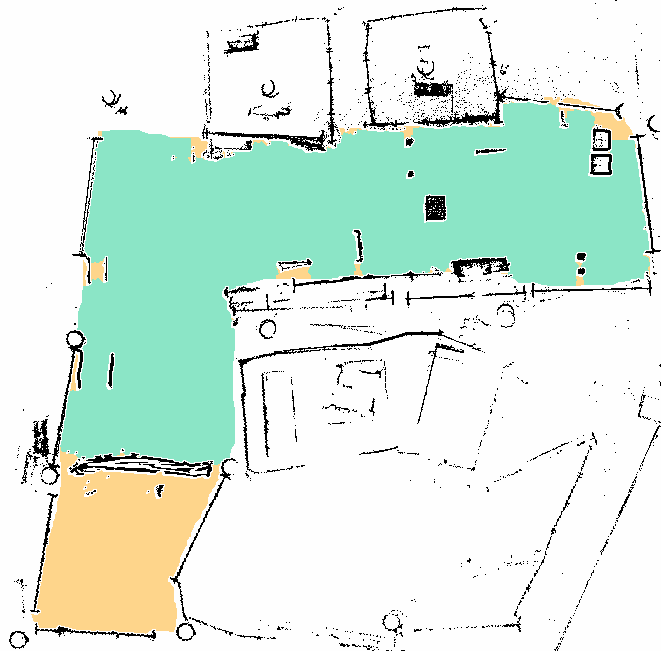
\includegraphics[width=0.31\textwidth]{figs/setting1_predicted.png}}\hfil
\subfloat[Annotated behaviour]{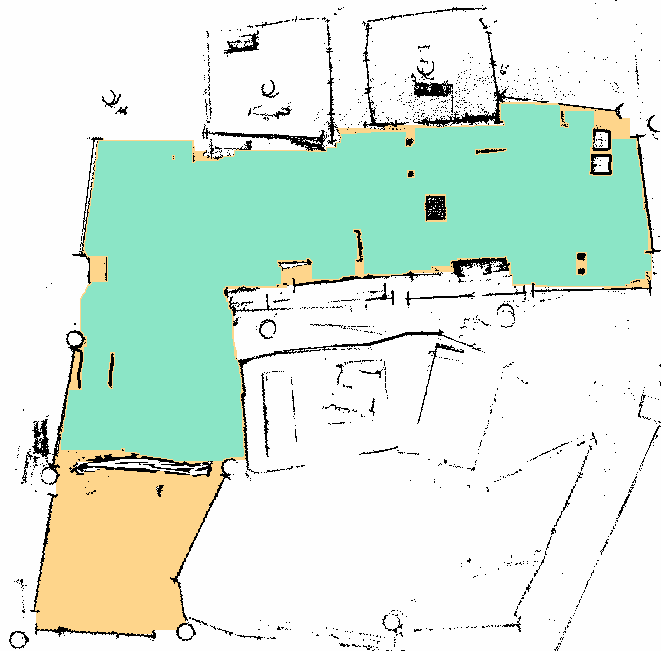
\includegraphics[width=0.31\textwidth]{figs/setting1_annotated.png}}\hfil
\subfloat[Disagreement]{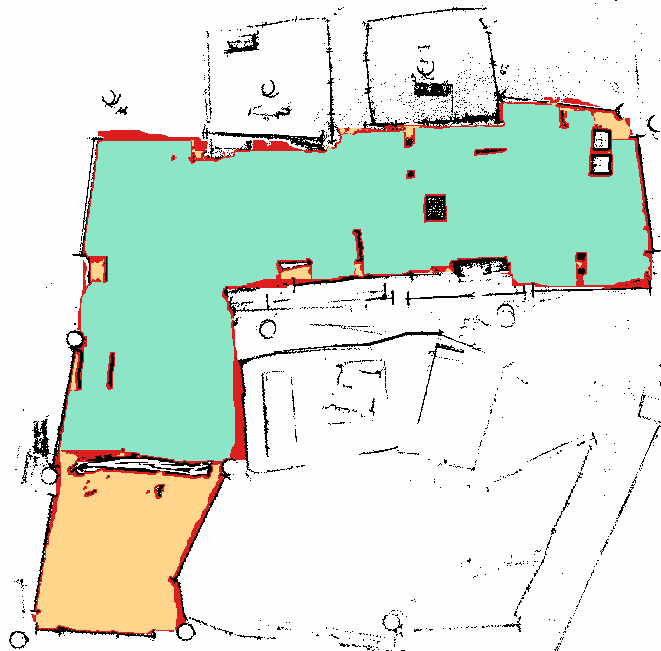
\includegraphics[width=0.31\textwidth]{figs/setting1_difference.png}}\\
\subfloat[Predicted]{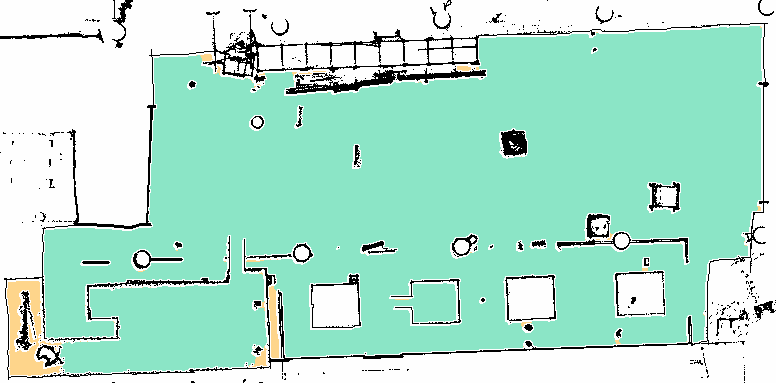
\includegraphics[width=0.31\textwidth]{figs/setting4_predicted.png}}\hfil
\subfloat[Annotated behaviour]{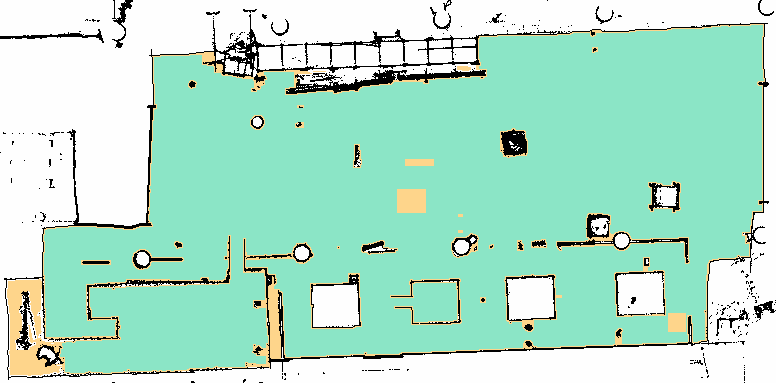
\includegraphics[width=0.31\textwidth]{figs/setting4_annotated.png}}\hfil
\subfloat[Disagreement]{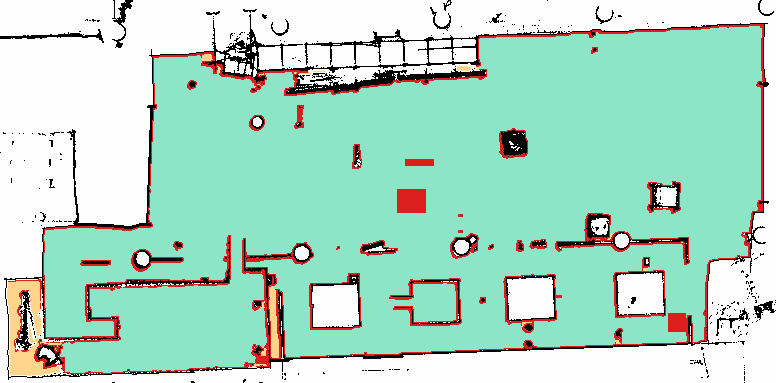
\includegraphics[width=0.31\textwidth]{figs/setting4_difference.png}}
\caption{Predicted accessibility heat maps compared with the maps annotated from observed robot behaviour, for Setting~1 with the Movilo (top row) and Setting~4 with the GO2 (bottom row). Green marks area the robot can reach and orange marks required area it cannot. The disagreement panels colour every pixel on which the two maps differ in red, showing that disagreement concentrates in a thin halo at the region boundaries rather than in the interior.}
\label{fig:heatmaps}
\end{figure*}
 
\subsection{Closed-Loop Site Improvement}
\label{sec:loop}
The closed loop of Section~\ref{sec:relocation} was exercised in four of the settings. In each test the framework computed the as-found index, the barrier diagnosis proposed the relocation of blocking obstacles, an operator refined and confirmed the plan in the interface, the site team applied the changes physically, and the audit robot rescanned the area for a second assessment. Table~\ref{tab:relocation} reports, for each test, the as-found index, the index predicted after the planned relocation, and the index measured from the repeat scan, and Fig.~\ref{fig:beforeafter} shows a representative pair of heat maps before and after the change.
% TODO fill tab:relocation from the four before and after tests
\textit{[Sentence to be added, the measured gains tracked the predicted gains within X percentage points across the four tests.]}
 
\begin{table}[t]
\caption{Closed-loop relocation tests, predicted and measured index.}
\label{tab:relocation}
\centering
\footnotesize
% TODO fill the four rows, values in percent
\begin{tabular}{@{}lcccc@{}}
\toprule
Test & Robot & As-found & Predicted after & Measured after \\
\midrule
R1 & \textit{[fill]} & & & \\
R2 & & & & \\
R3 & & & & \\
R4 & & & & \\
\bottomrule
\end{tabular}
\end{table}
 
\begin{figure}[t]
\centering
% TODO replace placeholder with a representative before and after pair
\framebox[\linewidth]{\rule{0pt}{3.2cm}\parbox{0.9\linewidth}{\centering Placeholder. Heat map of one setting before relocation beside the heat map after relocation, with the moved obstacles indicated.}}
\caption{Accessibility heat maps of one setting before and after the guided relocation, with the relocated obstacles indicated. The regained area corresponds to the gain reported in Table~\ref{tab:relocation}.}
\label{fig:beforeafter}
\end{figure}
 
\subsection{Discussion}
\label{sec:discussion}
Taken together, the experiments answer the three questions in order. On the settings quantified at pixel level, the maps the framework predicted matched the behaviour annotated from video on 92.4\% of the labelled area, and on 97.7\% once boundary rendering effects are set aside, so the heat maps can be read as faithful forecasts of where a platform will and will not operate. The platform differences appeared where the parameters place them, which supports assessing an entire fleet from a single scan. The relocation tests show that the predicted gains are actionable rather than notional, since gains forecast in the interface were realised on the physical site and confirmed by an independent rescan. % TODO temper or strengthen this sentence once the four deltas are in
Two limitations remain. Each assessment is a snapshot of a changing site, and all settings come from a single project, with four relocation tests forming a small sample. Broader validation across sites and larger intervention studies remain for future work.

\section*{Acknowledgment}

The preferred spelling of the word ``acknowledgment'' in America is without 
an ``e'' after the ``g''. Avoid the stilted expression ``one of us (R. B. 
G.) thanks $\ldots$''. Instead, try ``R. B. G. thanks$\ldots$''. Put sponsor 
acknowledgments in the unnumbered footnote on the first page.
\bibliographystyle{IEEEtran}
\bibliography{ref}


\end{document}
